\section{Thesis Proposal}
\label{sec:proposal}

The formal understanding of early warning signals of critical transitions requires future clarification; specifically, the current theory relies on long-term and linear approximations while ignoring transient behavior. 

One line of research seeks to clarify the effect of short term non-exponential behavior. For example, reactivity has recently been shown to change systematically leading up to bifurcation in a certain class of infectious disease models \cite{oreganTransientIndicatorsTipping2020}. 

On the other hand, I propose to clarify the effect of behavior far away from the attractor -- far enough that it is not within the descriptive bounds of a linear approximation. I suggest investigating the relationship between intensity of attraction and critical transitions. 
%
Toward this goal, I propose to relate intensity to at least three different aspects of tipping behavior: local bifurcations, tipping across basin boundaries, and reversibility of hysteretic transitions. As a supplementary pursuit, I would also like to improve the general theoretical understanding of intensity of attraction, by considering various open questions related to it. Finally, I will mention at the end of this section some further possible connections -- to machine learning based warning signals and a framework known as  flow-kick systems. 
%
Perhaps this work may eventually help build toward a theory of early warning indicators brought about by changes before a critical transition. 

%I would like to pursue analytic results as well as application-specific examples. 

%Propose some avenues that may help build toward a theory of early warning indicators brought about by changes in intensity during the time leading up to a critical transition. 
%
%Might be that intensity only provides useful warning indicators in a specific class of critical transitions, or for a specific class of ODEs. 

TO DO: Motivating example where intensity might be useful.

%\subsection{Continuity of Intensity}

%\subsection{Demographic Versus Environmental Perturbations}

\subsection{Intensity Through Local Bifurcations}

How does intensity of attraction behave when passing through a local bifurcation? Does it display a systematic change, similar to the way that asymptotic resilience? 

Why does this matter? Connect back to motivation. 

Here, a first step may be to prove continuity of intensity with respect to parameter changes. 

\begin{conjecture}(McGehee or Meyer?)
	Intensity is continuous with respect to parameter changes. To do: phrase this formally. What might be the right way?
\end{conjecture}

Next, I would investigate one dimensional saddle-node, transcritical, and pitchfork bifurcations. 
%
Start with numerical computations of intensity across application-specific examples of bifurcation. Then try to prove analytic results. 
%
I think in these bifurcation types, intensity should go to zero. In some systems intensity may decrease at a similar or proportional rate as does asymptotic resilience. But in others, their two rates of decrease may not be as straightforwardly related. 

Why do I think this? Provide justification.

%Some authors have argued that another basin-based measure of resilience, basin-width, is linearly related to asymptotic resilience -- to do: cite and check if the phrasing is correct. 

Also, Hopf bifurcations. Could start with Kate's generalized Lotka-Volterra example and do a numerical simulation. %Not really sure what to expect here in general. 

%Maybe nothing interesting?

"Critical widening"? Not explained by critical slowing down with state variable perturbation. But can be explained by decreasing intensity leading up to bifurcation with vector field perturbation. In reality perturbations may be a combination of state and vector field perturbations (e.g. demographic and environmental perturbations).

\subsection{Tipping Across Basin Boundaries}

Critical slowing down pertains only to only to one specific category of tipping behavior – local bifurcations. But another class of tipping behavior occurs when perturbations push a state variable into an alternative basin of attraction. Intensity measures how difficult it is for this type of tipping to occur under bounded control types of perturbations. (Many other dynamical behaviors also correspond to tipping, and are not considered here, including global bifurcations, rate-induced tipping, and transitions to chaotic regimes.)

Mention flickering & skewness indicators. But these are also understood on from an informal point of view, with a unclear formal basis. 

\subsection{Reversibility of Hysteretic Transitions}

Explain what hysteresis is and give example of hysteresis. Figure (\ref{fig:hysteresis}).

\begin{figure}[ht]
	\centering
	\captionsetup{width=0.4\linewidth}
	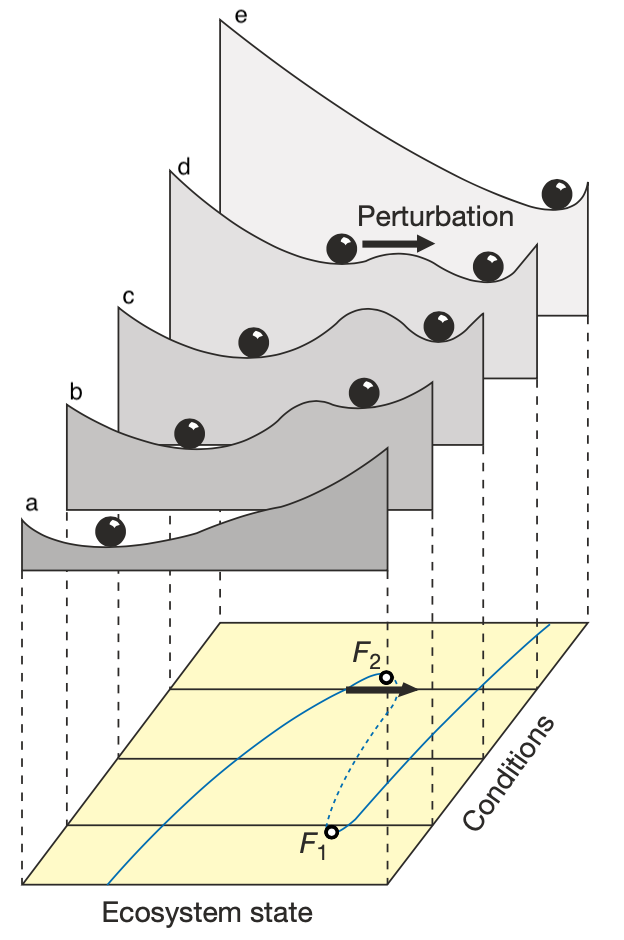
\includegraphics[width=0.4\textwidth]{figs/hysteresis}
	\caption{Hysteresis. Figure reproduced from \cite{schefferCatastrophicShiftsEcosystems2001a}.}
	
	\label{fig:hysteresis}
\end{figure} 

%At least two types: cubic type or parabolic plus additional steady state type (e.g. KIausmeier equation)

Intensity of the alternative attractors describes whether the basin boundary tends to be crossed before the bifurcation point or not. 
%
Could give a measure of how reversible the bifurcation is -- from completely hysteretic to much more easily reversible than the bifurcation diagram would suggest. 

Is it useful to define an analog of intensity for the repeller in between the alternative attractors?

\subsection{General Open Questions About Intensity}

\subsubsection{Estimates of Intensity}
One basic limitation of using intensity of attraction in any application right now: numerical computations of intensity (which currently use set-valued Euler methods on a fixed grid) are too time-intensive. Instead, analytic tools should be developed that can be used for estimating intensity. (There is also a need for improved numerical methods, although this important avenue is not the focus of my thesis proposal.) For instance, I would start by pursuing a proof of Conjecture \ref{conj:steepness}, which may provide a tractable way to estimate a lower bound on intensity without requiring a full numerical computation. 

\subsubsection{Critical Reachable Set}

What is the smallest set $A \subset N \subset basin(A)$ so that if $N \subset R_r(A)$ then $intensity(A) \leq r$?

In other words, if under $r$-bounded control you can reach $N$ then you can escape the basin. This is a critical set in the sense that it is the "hardest" part of the basin to overcome -- once you can reach $N$ then you can leave the basin. 

\subsection{Further Possibilities}

Machine learning based early warning signals? Possible connection between machine-learning based and analytical theory based early warning signals? i.e. using theory to inform ML design. 

%Validating on actual data from somewhere?

Connections to Flow-Kick systems? What about connections to multiflows?

